\documentclass[11pt]{article}
\usepackage[letterpaper]{geometry}
\usepackage{url}
\usepackage{salgorithm}
\usepackage{graphicx} \graphicspath{{sorts/}}



\title{A Simple and Useful Model of Virtual Memory Performance}
\author{Peter Boothe\\
Manhattan College\\
\url{peter.boothe@manhattan.edu}
}
\date{Submission to ALENEX2011}

\newcommand{\heapsort}{{\sc HeapSort}}
\newcommand{\quicksort}{{\sc QuickSort}}
\newcommand{\mergesort}{{\sc MergeSort}}
\newcommand{\NAA}{\textrm{NAA}}

\begin{document}
\maketitle

As memory requirements begin to outstrip available memory on a machine, the
operating system will allocate virtual memory to supplement the available
physical memory.  We present, argue for, and experimentally validate a simple
model and analysis technique which allows algorithm developers to analyze the
behavior of an algorithm when virtual memory is used.  In particular, the
penalty for a page fault in virtual memory can be extreme, and can make
previously-small constants quite large. Thus, it would be of great use to be
able to easily estimate, for a given algorithm, the number of times the
algorithm will have to wait for the operating system to retrieve virtual memory
pages off the hard drive.

\section{The Method}

In the worst case, every memory access will have to go to the hard drive.
This, however, is not an informative worst-case analysis.  The worst-case page
fault predictions do not reflect the real-world behavior of virtual memory ---
they reflect a situation in which every cache access is a cache miss! Our
model predicts that all non-adjacent memory accesses have a uniform non-zero probability of causing a page fault. 

Our method of estimating the number of page faults is therefore to count the
number of non-adjacent memory accesses.  Using this, we find that we also end
up providing a quantitative measure of ``cache friendliness'', which is a term
often used, but seldom rigorously defined.  We demonstrate our method
using three classic sorting techniques: \heapsort, \quicksort, and \mergesort.


\subsection{\heapsort\ Page Fault Analysis}
Our analysis of \heapsort\ is the easiest.  The \heapsort\ algorithm, which we
take from Cormen {\it et al.}\cite{clrs}, is defined, with all of its
supporting functions, in Figure~\ref{fig:hsort}.  The implementation we tested
is from the BSD standard library, and libbsd on Linux.

\begin{figure}
\begin{algorithm}
\Algorithm{HeapSort}$(array, size)$\+\\
    Build-Max-Heap$(array, size)$\\
    \For $i \gets size$ \DownTo\ $2$\+\\
        exchange $array[1] \leftrightarrow array[i]$\\
        $size \gets size - 1$\\
        Max-Heapify$(array, 1, size)$\-\\
    \Return $array$\-\\
\\
\Algorithm{Build-Max-Heap}$(array, size)$\+\\
    \For $i \gets \lfloor \frac{size}{2} \rfloor$ \DownTo\ $1$\+\\
        Max-Heapify$(array, i, size)$\-\-\\
\\
\Algorithm{Max-Heapify}$(array, i, size)$\+\\
    $l \gets 2*i$\\
    $r \gets 2*i + 1$\\
    $largest \gets i$\\
    \If $l < size$ and $array[l] > array[largest]$\+\\
            $largest \gets l$\-\\
    \If $r < size$ and $array[r] > array[largest]$\+\\
            $largest \gets r$\-\\
    \If $largest \neq i$\+\\
        exchange $array[i] \leftrightarrow array[largest]$\\
        Max-Heapify$(array, largest, size)$
\end{algorithm}

\caption{\heapsort\ from Cormen {\it et al.}\cite{clrs}.}
\label{fig:hsort}
\end{figure}

In the pseudocode of \heapsort, we note that, with the exception of the very
top of the heap, at no point do we ever access memory adjacent to the most
recently used memory location.  Therefore, we predict that the number of page
faults will be proportional to the number of memory accesses, which in the case
of \heapsort\ is proportional to its runtime of $O(n \log n)$.

\subsection{\mergesort\ Page Fault Analysis} 

The \mergesort\ algorithm we take from Cormen {\it et al.}\cite{clrs} with the
memory-efficiency improvement that we only copy out the first half of the
array.  Our implementation, in its entirety, may be found in
Figure~\ref{fig:msort}.  In our analysis, the only consideration is the number
and location of memory accesses, and memory accesses only occur in the
``merge'' portion of the algorithm.

\begin{figure}
\begin{verbatim}
void mergesort(int array[], long lo, long hi)
{
    int *spare;
    int ssize;
    long sindex, hindex;
    long mid;

    // Base case
    if (lo+1 >= hi) return; 

    // Recurse on each half
    mid = (lo + hi) / 2;  
    mergesort(array, lo, mid);
    mergesort(array, mid, hi);

    // Merge
    ssize = mid-lo; // Only copy out the first half
    spare = (int *)malloc(ssize * sizeof(int));
    memcpy(spare, &(array[lo]), ssize * sizeof(int));

    sindex = 0;
    hindex = mid;
    while (sindex < ssize && hindex < hi) {
        if (spare[sindex] < array[hindex])
            array[lo++] = spare[sindex++];
        else
            array[lo++] = array[hindex++];
    }

    while (sindex < ssize) array[lo++] = spare[sindex++];

    free(spare);
}
\end{verbatim}


\caption{Our \mergesort\ implementation in its entirety.}
\label{fig:msort}
\end{figure}

In merging, the first step is to allocate a new array of size equal to half of
the passed-in array.  Then, the first half of the passed-in array is copied to
the new array.  The copying is done by accessing consecutive elements of each
array, and so once the beginning of each array has been accessed, all subsequent memory accesses are adjacent.  Therefore, the initial step has two non-adjacent accesses.

Subsequently, we treat the latter half of the passed-in array as one queue, and the newly-allocated array as the second queue.  We then merge by repeatedly removing the smaller item from the front of the two queues and overwriting an element of the passed-in array.  Every examination requires a memory access, but in all cases except the initial examination of the fronts of the queues, all memory accesses occur adjacent to previous memory accesses.  Therefore, to merge the newly-allocated array and the passed-in array requires two non-adjacent memory accesses.  In total, each call to our \mergesort function can require four non-adjacent memory accesses.

Over the whole of the algorithm, we find that the number
of non-adjacent accesses for \mergesort on an array of size $n$ ($\NAA(n)$) is $$\NAA(n) = 4 + 2\NAA(\frac{n}{2})$$
By the master theorem, we can see that $\NAA(n) \in \Theta(n)$, and
we therefore expect the number of page faults to grow linearly with the
size of the input to \mergesort.

\section{Experimental Validation of Our Model's Conclusions}

An experimental model can not be verified to be correct, it can only be shown
that the available tests do not prove the model wrong.  Here, we construct a
set of tests which repeatedly fail to disprove our model.

\subsection{Experimental Setup}

To analyze the number of major page faults in an algorithm, we must run our
algorithm in low-memory conditions so that the operating system is forced to
allocate and use virtual memory for our program.  Unfortunately, accessing swap
is incredibly slow --- a major part of the motivation for our study --- which
means that under low-memory conditions our tests may require 100x more time to
finish.  

We reconcile the opposing forces by running our tests in a virtual machine via
the Qemu emulator.  The machine which is running the emulator was given 4
gigabytes of memory.  Of those 4 Gb, half of it was allocated to be a RAM disk.
The swap partition of the emulated machine was a file stored on that RAM disk.
This meant that the page faults of the emulated machine would still be
recorded, but that the emulated machine would not suffer a performance hit, as
the emulated swap was backed by an extremely fast RAM disk!  We recommend this
technique for anyone who would like to count page faults but does not want to
waste a lot of time.

Interestingly, the RAM disk turned out to be helpful, but not essential, as the
natural caching behaviour of the host operating system meant that even when the
emulated swap was backed by a physical hard drive, it was often cached in the
memory of the host operating system.

\subsection{\heapsort}

\subsection{\mergesort}

\subsection{Number of Page Faults Compared}

\begin{figure}
% GNUPLOT: LaTeX picture with Postscript
\begingroup
  \makeatletter
  \providecommand\color[2][]{%
    \GenericError{(gnuplot) \space\space\space\@spaces}{%
      Package color not loaded in conjunction with
      terminal option `colourtext'%
    }{See the gnuplot documentation for explanation.%
    }{Either use 'blacktext' in gnuplot or load the package
      color.sty in LaTeX.}%
    \renewcommand\color[2][]{}%
  }%
  \providecommand\includegraphics[2][]{%
    \GenericError{(gnuplot) \space\space\space\@spaces}{%
      Package graphicx or graphics not loaded%
    }{See the gnuplot documentation for explanation.%
    }{The gnuplot epslatex terminal needs graphicx.sty or graphics.sty.}%
    \renewcommand\includegraphics[2][]{}%
  }%
  \providecommand\rotatebox[2]{#2}%
  \@ifundefined{ifGPcolor}{%
    \newif\ifGPcolor
    \GPcolortrue
  }{}%
  \@ifundefined{ifGPblacktext}{%
    \newif\ifGPblacktext
    \GPblacktexttrue
  }{}%
  % define a \g@addto@macro without @ in the name:
  \let\gplgaddtomacro\g@addto@macro
  % define empty templates for all commands taking text:
  \gdef\gplbacktext{}%
  \gdef\gplfronttext{}%
  \makeatother
  \ifGPblacktext
    % no textcolor at all
    \def\colorrgb#1{}%
    \def\colorgray#1{}%
  \else
    % gray or color?
    \ifGPcolor
      \def\colorrgb#1{\color[rgb]{#1}}%
      \def\colorgray#1{\color[gray]{#1}}%
      \expandafter\def\csname LTw\endcsname{\color{white}}%
      \expandafter\def\csname LTb\endcsname{\color{black}}%
      \expandafter\def\csname LTa\endcsname{\color{black}}%
      \expandafter\def\csname LT0\endcsname{\color[rgb]{1,0,0}}%
      \expandafter\def\csname LT1\endcsname{\color[rgb]{0,1,0}}%
      \expandafter\def\csname LT2\endcsname{\color[rgb]{0,0,1}}%
      \expandafter\def\csname LT3\endcsname{\color[rgb]{1,0,1}}%
      \expandafter\def\csname LT4\endcsname{\color[rgb]{0,1,1}}%
      \expandafter\def\csname LT5\endcsname{\color[rgb]{1,1,0}}%
      \expandafter\def\csname LT6\endcsname{\color[rgb]{0,0,0}}%
      \expandafter\def\csname LT7\endcsname{\color[rgb]{1,0.3,0}}%
      \expandafter\def\csname LT8\endcsname{\color[rgb]{0.5,0.5,0.5}}%
    \else
      % gray
      \def\colorrgb#1{\color{black}}%
      \def\colorgray#1{\color[gray]{#1}}%
      \expandafter\def\csname LTw\endcsname{\color{white}}%
      \expandafter\def\csname LTb\endcsname{\color{black}}%
      \expandafter\def\csname LTa\endcsname{\color{black}}%
      \expandafter\def\csname LT0\endcsname{\color{black}}%
      \expandafter\def\csname LT1\endcsname{\color{black}}%
      \expandafter\def\csname LT2\endcsname{\color{black}}%
      \expandafter\def\csname LT3\endcsname{\color{black}}%
      \expandafter\def\csname LT4\endcsname{\color{black}}%
      \expandafter\def\csname LT5\endcsname{\color{black}}%
      \expandafter\def\csname LT6\endcsname{\color{black}}%
      \expandafter\def\csname LT7\endcsname{\color{black}}%
      \expandafter\def\csname LT8\endcsname{\color{black}}%
    \fi
  \fi
  \setlength{\unitlength}{0.0500bp}%
  \begin{picture}(7200.00,5040.00)%
    \gplgaddtomacro\gplbacktext{%
      \csname LTb\endcsname%
      \put(1606,1144){\makebox(0,0)[r]{\strut{} 0}}%
      \csname LTb\endcsname%
      \put(1606,1747){\makebox(0,0)[r]{\strut{} 200000}}%
      \csname LTb\endcsname%
      \put(1606,2350){\makebox(0,0)[r]{\strut{} 400000}}%
      \csname LTb\endcsname%
      \put(1606,2954){\makebox(0,0)[r]{\strut{} 600000}}%
      \csname LTb\endcsname%
      \put(1606,3557){\makebox(0,0)[r]{\strut{} 800000}}%
      \csname LTb\endcsname%
      \put(1606,4160){\makebox(0,0)[r]{\strut{} 1e+06}}%
      \csname LTb\endcsname%
      \put(1738,924){\makebox(0,0){\strut{} 0}}%
      \csname LTb\endcsname%
      \put(2671,924){\makebox(0,0){\strut{} 200}}%
      \csname LTb\endcsname%
      \put(3604,924){\makebox(0,0){\strut{} 400}}%
      \csname LTb\endcsname%
      \put(4537,924){\makebox(0,0){\strut{} 600}}%
      \csname LTb\endcsname%
      \put(5470,924){\makebox(0,0){\strut{} 800}}%
      \csname LTb\endcsname%
      \put(6403,924){\makebox(0,0){\strut{} 1000}}%
      \put(440,2652){\rotatebox{90}{\makebox(0,0){\strut{}Number of major page faults}}}%
      \put(4304,594){\makebox(0,0){\strut{}Problem size in megabytes}}%
      \put(4304,4710){\makebox(0,0){\strut{}Problem size vs Page Faults}}%
      \put(4304,4490){\makebox(0,0){\strut{}Each line holds available memory constant}}%
    }%
    \gplgaddtomacro\gplfronttext{%
      \csname LTb\endcsname%
      \put(3449,173){\makebox(0,0)[r]{\strut{}Heapsort}}%
      \csname LTb\endcsname%
      \put(5492,173){\makebox(0,0)[r]{\strut{}Mergesort}}%
    }%
    \gplbacktext
    \put(0,0){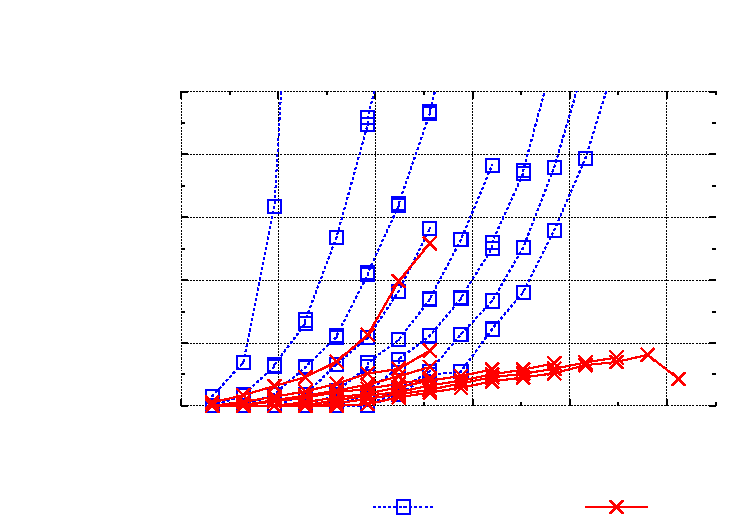
\includegraphics{memsizes}}%
    \gplfronttext
  \end{picture}%
\endgroup

\caption{Number of major page faults for \mergesort\ and \heapsort\ at a variety of memory sizes.  Note that at almost all memory sizes, \mergesort\ is better.}
\end{figure}

\begin{figure}
% GNUPLOT: LaTeX picture with Postscript
\begingroup
  \makeatletter
  \providecommand\color[2][]{%
    \GenericError{(gnuplot) \space\space\space\@spaces}{%
      Package color not loaded in conjunction with
      terminal option `colourtext'%
    }{See the gnuplot documentation for explanation.%
    }{Either use 'blacktext' in gnuplot or load the package
      color.sty in LaTeX.}%
    \renewcommand\color[2][]{}%
  }%
  \providecommand\includegraphics[2][]{%
    \GenericError{(gnuplot) \space\space\space\@spaces}{%
      Package graphicx or graphics not loaded%
    }{See the gnuplot documentation for explanation.%
    }{The gnuplot epslatex terminal needs graphicx.sty or graphics.sty.}%
    \renewcommand\includegraphics[2][]{}%
  }%
  \providecommand\rotatebox[2]{#2}%
  \@ifundefined{ifGPcolor}{%
    \newif\ifGPcolor
    \GPcolorfalse
  }{}%
  \@ifundefined{ifGPblacktext}{%
    \newif\ifGPblacktext
    \GPblacktexttrue
  }{}%
  % define a \g@addto@macro without @ in the name:
  \let\gplgaddtomacro\g@addto@macro
  % define empty templates for all commands taking text:
  \gdef\gplbacktext{}%
  \gdef\gplfronttext{}%
  \makeatother
  \ifGPblacktext
    % no textcolor at all
    \def\colorrgb#1{}%
    \def\colorgray#1{}%
  \else
    % gray or color?
    \ifGPcolor
      \def\colorrgb#1{\color[rgb]{#1}}%
      \def\colorgray#1{\color[gray]{#1}}%
      \expandafter\def\csname LTw\endcsname{\color{white}}%
      \expandafter\def\csname LTb\endcsname{\color{black}}%
      \expandafter\def\csname LTa\endcsname{\color{black}}%
      \expandafter\def\csname LT0\endcsname{\color[rgb]{1,0,0}}%
      \expandafter\def\csname LT1\endcsname{\color[rgb]{0,1,0}}%
      \expandafter\def\csname LT2\endcsname{\color[rgb]{0,0,1}}%
      \expandafter\def\csname LT3\endcsname{\color[rgb]{1,0,1}}%
      \expandafter\def\csname LT4\endcsname{\color[rgb]{0,1,1}}%
      \expandafter\def\csname LT5\endcsname{\color[rgb]{1,1,0}}%
      \expandafter\def\csname LT6\endcsname{\color[rgb]{0,0,0}}%
      \expandafter\def\csname LT7\endcsname{\color[rgb]{1,0.3,0}}%
      \expandafter\def\csname LT8\endcsname{\color[rgb]{0.5,0.5,0.5}}%
    \else
      % gray
      \def\colorrgb#1{\color{black}}%
      \def\colorgray#1{\color[gray]{#1}}%
      \expandafter\def\csname LTw\endcsname{\color{white}}%
      \expandafter\def\csname LTb\endcsname{\color{black}}%
      \expandafter\def\csname LTa\endcsname{\color{black}}%
      \expandafter\def\csname LT0\endcsname{\color{black}}%
      \expandafter\def\csname LT1\endcsname{\color{black}}%
      \expandafter\def\csname LT2\endcsname{\color{black}}%
      \expandafter\def\csname LT3\endcsname{\color{black}}%
      \expandafter\def\csname LT4\endcsname{\color{black}}%
      \expandafter\def\csname LT5\endcsname{\color{black}}%
      \expandafter\def\csname LT6\endcsname{\color{black}}%
      \expandafter\def\csname LT7\endcsname{\color{black}}%
      \expandafter\def\csname LT8\endcsname{\color{black}}%
    \fi
  \fi
  \setlength{\unitlength}{0.0500bp}%
  \begin{picture}(7200.00,5040.00)%
    \gplgaddtomacro\gplbacktext{%
      \csname LTb\endcsname%
      \put(1078,704){\makebox(0,0)[r]{\strut{} 0}}%
      \csname LTb\endcsname%
      \put(1078,1568){\makebox(0,0)[r]{\strut{} 5}}%
      \csname LTb\endcsname%
      \put(1078,2432){\makebox(0,0)[r]{\strut{} 10}}%
      \csname LTb\endcsname%
      \put(1078,3296){\makebox(0,0)[r]{\strut{} 15}}%
      \csname LTb\endcsname%
      \put(1078,4160){\makebox(0,0)[r]{\strut{} 20}}%
      \csname LTb\endcsname%
      \put(1210,484){\makebox(0,0){\strut{} 0}}%
      \csname LTb\endcsname%
      \put(1725,484){\makebox(0,0){\strut{} 100}}%
      \csname LTb\endcsname%
      \put(2239,484){\makebox(0,0){\strut{} 200}}%
      \csname LTb\endcsname%
      \put(2754,484){\makebox(0,0){\strut{} 300}}%
      \csname LTb\endcsname%
      \put(3268,484){\makebox(0,0){\strut{} 400}}%
      \csname LTb\endcsname%
      \put(3783,484){\makebox(0,0){\strut{} 500}}%
      \csname LTb\endcsname%
      \put(4297,484){\makebox(0,0){\strut{} 600}}%
      \csname LTb\endcsname%
      \put(4812,484){\makebox(0,0){\strut{} 700}}%
      \csname LTb\endcsname%
      \put(5326,484){\makebox(0,0){\strut{} 800}}%
      \csname LTb\endcsname%
      \put(5841,484){\makebox(0,0){\strut{} 900}}%
      \csname LTb\endcsname%
      \put(6355,484){\makebox(0,0){\strut{} 1000}}%
      \csname LTb\endcsname%
      \put(6870,484){\makebox(0,0){\strut{} 1100}}%
      \put(440,2432){\rotatebox{90}{\makebox(0,0){\strut{}Ratio of Heapsort page faults to Mergesort page faults}}}%
      \put(4040,154){\makebox(0,0){\strut{}Problem size in megabytes}}%
      \put(4040,4710){\makebox(0,0){\strut{}Heapsort is bad and gets worse as problems grow}}%
      \put(4040,4490){\makebox(0,0){\strut{}Each line holds available memory constant}}%
    }%
    \gplgaddtomacro\gplfronttext{%
    }%
    \gplbacktext
    \put(0,0){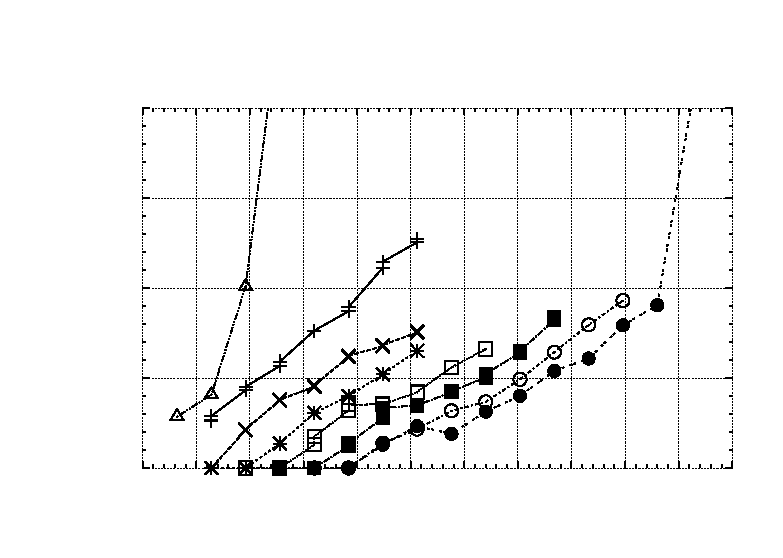
\includegraphics{ratios}}%
    \gplfronttext
  \end{picture}%
\endgroup

\caption{Number major page faults for \heapsort\ divided by the number of major page faults for \mergesort\ at a variety of memory sizes.  The fact that this ratio grows over time indicates the \heapsort\ has asymptotically more page faults than \mergesort, which is exactly what is predicted by our model!}
\end{figure}

\section{Conclusion}

\bibliographystyle{abbrv}
\bibliography{bibliography}

\end{document}
